\chapter{Additional Chapter}

\section{$\mathbb{S}^1 \times \mathbb{S}^1 \not\cong \mathbb{S}^2$}

\subsection{Method 1: Euler Characteristic}

\subsection{Method 2: Simple Closed Curve}

\begin{definition}{Simple Closed Curve (SCC)}\\
A SCC in a topological space $X$ is a set $C \subseteq X$, s.t.: there exists a homeomorphism $h: \mathbb{S}^1 \rightarrow C$.
\end{definition}

\begin{theorem}{Jordan Curve Theorem}\\
If $C$ is a SCC in $\mathbb{R}^2$, then $\mathbb{R}^2 - C$ has exactly two path-connected components.
\end{theorem}

\noindent\textbf{Remark:} Since $\mathbb{R}^2 \cup \{ \infty \}\cong \mathbb{S}^2$, then we have the following corollary.

\begin{corollary}{Sphere version of Jordan Curve Theorem}\\
If $C$ is a SCC in $\mathbb{S}^2$, then $\mathbb{S}^2 - C$ has exactly two path-connected components.
\end{corollary}

\begin{proposition}
    Let $f: X \overset{\cong}{\rightarrow} Y$ be a homeomorphism. $f(C)$ is a SCC if $C$ is a SCC.
\end{proposition}

\begin{proof}
    Let $h: \mathbb{S}^1 \overset{\cong}{\rightarrow} C (\subseteq X)$ be a homeomorphism by the def of SCC. Then it's easy to show that $f \circ h$ is a homeomorphism between $\mathbb{S}^1 \cong f(C)$.
\end{proof}

\begin{proposition}
    For any $p\in \mathbb{S}^1$, define 
    $$\gamma_p := \mathbb{S}^1 \times \{ p\}.$$
    Then we have:
    $$\mathbb{T}^2 - \gamma_p \cong \mathbb{S}^1 \times (0,1).$$
\end{proposition}

\begin{proposition}
    $$\mathbb{S}^1 \times \mathbb{S}^1 \not\cong \mathbb{S}^2$$
\end{proposition}

\begin{proof}
    Suppose on the contrary that $\mathbb{S}^1 \times \mathbb{S}^1 \cong \mathbb{S}^2$. Then $\mathbb{T}^2 \cong \mathbb{S}^2$. Then there is a homeomorphism $f:\mathbb{S}^2 \overset{\cong}{\rightarrow} \mathbb{T}^2$.

    By proposition 1.4 and 1.5, $f^{-1}(\gamma_0)$ is NOT a SCC in $\mathbb{S}^2$. Hence, $f^{-1}(\gamma_0) = \{ q\}$ for some $q \in \partial \mathbb{S}^2$, contradicting the infectivity of $f$.
\end{proof}

\section{Computing $\Pi_1 (X)$}

\subsection{Dimensionality Reduction}

\begin{definition}
    Let $X$ be a topological space, $A \subseteq X$ and let $i: A \to X$ be an inclusion. 
    \begin{itemize}
        \item We say $A$ is a \textit{homotopy retract (deformation retract)} of $X$, if there exists a continuous map $r: X \rightarrow A$, s.t.:
        \begin{align*}
            &r \circ i: A \overset{i}{\rightarrow} X \overset{r}{\rightarrow} A = id_A\\
            &i \circ r : X \overset{r}{\rightarrow} A \overset{i}{\rightarrow} X \simeq id_X
        \end{align*}
        Moreover, we call $r$ here is a retraction. Furthermore, for all $a \in A$, $$r(a) = a$$
        \item If $r: X \to A$ is a retraction, then there exists a homotopy $H : X \times I \to X$, s.t.: $H(x,0) =x$, $H(x,1)=r(x)$ and $H(a,t) = a$ for any $a \in A$, $t\in I$.
    \end{itemize}
\end{definition}

\begin{proposition}
    If $A$ is a deformation retract of $X$, then
    $$A \simeq X$$
\end{proposition}

\noindent\textbf{Example:} 
\begin{itemize}
    \item For any point $p \in \mathbb{S}^n$, $\{p\}$ is a deformation retract, i.e.:
    $$\Pi_1(\mathbb{S}^n) \cong \Pi_1(\{p\}) =\{e\}$$
    which follows that $\mathbb{S}^n$ is simply-connected.
    \item $\mathbb{S}^1$ is a deformation retract of $X:= \mathbb{R}^2 \setminus \{0\}$.
    \begin{proof}
        Consider $r: \mathbb{R}^2 \setminus \{0\} \to \mathbb{S}^1$ given by
        $$r(\mathbf{x}) := \frac{\mathbf{x}}{||\mathbf{x}||}$$
        It's easy to check that $r$ is continuous. Then construct $H: X \times I \to X$ by
        $$H(\mathbf{x},t) := (1-t) \mathbf{x} + t \cdot \frac{\mathbf{x}}{|| \mathbf{x}||}$$
        It remains to check that $H(\mathbf{x},t) \neq 0$ for all $\mathbf{x} \in X,t\in I$ for showing the well-defined-ness of $H$. Then one can find
        \begin{align*}
            &H(\mathbf{x},0) = \mathbf{x} =id_X(\mathbf{x}),H(\mathbf{x},1) = \frac{\mathbf{x}}{|| \mathbf{x}||} = r(\mathbf{x}) \;\;\forall \mathbf{x} \in X\\
            &\forall \mathbf{x} \in X, ||\mathbf{x}|| =1 \Rightarrow H(\mathbf{x},t) = (1-t) \mathbf{x} + t\mathbf{x} = \mathbf{x} \;\;\forall t \in I
        \end{align*}
        Therefore, $X$ can deformation retract to $\mathbb{S}^1$.
    \end{proof}
\end{itemize}

\begin{proposition}
    Let $X$ be a topological space, $A \subseteq X$, $x_0 \in X$ and let $i: A \rightarrow X$ be an inclusion map. If $A$ is a retract of $X$, then $i$ can induce a group homomorphism $i_* : \Pi_1 (A,x_0) \to \Pi_1 (X,x_0)$ is injective.
\end{proposition}

\begin{proof}
    \begin{equation*}
        (r \circ i)_* = r_* \circ i_* = (id_A)_* = id_{\Pi_1 (A,x_0)} \tag{\#}
    \end{equation*}
    For any $[l],[l'] \in \Pi_1 (A,x_0)$, if $i_*[l] = i_*[l']$, then
    $$[l] \overset{(\#)}{=} r_*(i_*[l]) = r_*(i_*[l']) \overset{(\#)}{=} [l']$$
    Therefore, $i_*$ is injective.
\end{proof}

\subsection{Dimensionality Raise}

\begin{definition}
    Let $X$ be a topological space.
    \begin{itemize}
        \item \textit{Cone}
        $$CX:= (X \times I) / (X \times \{1\})$$
        \item \textit{Suspension}
        $$SX:= (X \times I) / (X \times \{1\} \cup X \times \{0\})$$
    \end{itemize}
\end{definition}

\noindent\textbf{Example:} $$S(\mathbb{S}^n) \cong \mathbb{S}^{n+1}$$

\begin{proposition}
    For all topological space $X$, $CX$ is \textit{contractible}.
\end{proposition}

\begin{proof}
    Consider $H: CX \times I \to CX$ given by
    $$H([x,s],t) := [x,st]\;\;\forall $$
    Then 
    \begin{align*}
        &H([x,s],0) =[x,0] 
        \\&H([x,s],1) = [x,s] = id_{CX}([x,s])
    \end{align*}
    Hence, $H$ gives a homotopy between $id_{CX}$ and $c_{\{*\}}$ where $c_{\{*\}}$ denotes the constant map on the top of the cone, i.e.: $CX$ is contractible.
\end{proof}

\noindent\textbf{Example:} $$S (\mathbb{S}^0 := \{-1,1\}) =\mathbb{S}^1$$
\begin{proof}
    $S(\mathbb{S}^0) := \{-1,1\} \times I/ (\{-1,1\} \times \{1\} \cup \{-1,1\} \times \{0\})$
    \begin{figure}[htbp]
    \centering
    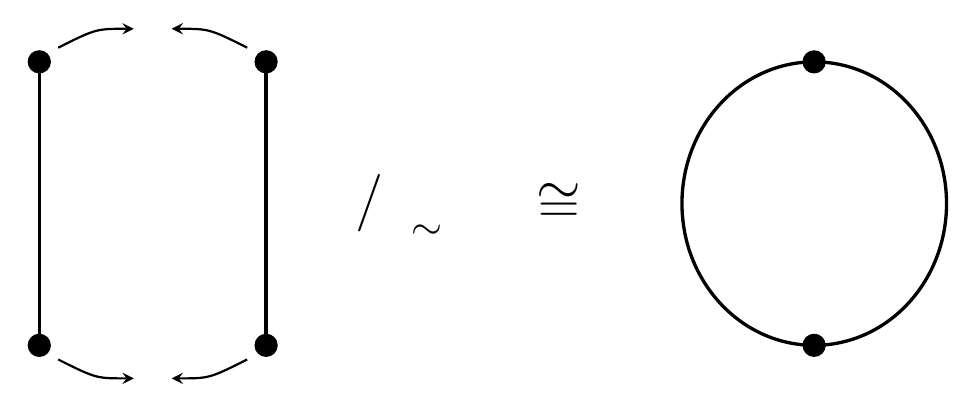
\begin{tikzpicture}[scale=1.2, very thick]
        
        \coordinate (TL) at (-1.2, 1.5); % Top Left
        \coordinate (BL) at (-1.2, -1.5); % Bottom Left
        \coordinate (TR) at (1.2, 1.5);  % Top Right
        \coordinate (BR) at (1.2, -1.5);  % Bottom Right

        
        \draw (TL) -- (BL);
        \draw (TR) -- (BR);

        
        \fill (TL) circle (3.5pt);
        \fill (BL) circle (3.5pt);
        \fill (TR) circle (3.5pt);
        \fill (BR) circle (3.5pt);

        
        \draw[->, >=stealth, thick] (-1.0, 1.65) .. controls (-0.6, 1.85) .. (-0.2, 1.85);
        \draw[->, >=stealth, thick] (1.0, 1.65) .. controls (0.6, 1.85) .. (0.2, 1.85);
        
        \draw[->, >=stealth, thick] (-1.0, -1.65) .. controls (-0.6, -1.85) .. (-0.2, -1.85);
        \draw[->, >=stealth, thick] (1.0, -1.65) .. controls (0.6, -1.85) .. (0.2, -1.85);

        
        \node at (2.3, 0) {\huge $/$};
        \node at (2.9, -0.3) {\Large $\sim$};
        
        
        \node at (4.3, 0) {\huge $\cong$};

        
        \coordinate (Center) at (7, 0);
        \draw (Center) circle[x radius=1.4, y radius=1.5];
        
        
        \fill (7, 1.5) circle (3.5pt);
        \fill (7, -1.5) circle (3.5pt);

    \end{tikzpicture}
    
\end{figure}
\end{proof}

\subsection{Exercise}

\begin{exercise}
    $X \subseteq \mathbb{R}^3$, $X$ be union of $n$ lines through the origin, compute $\Pi_1 (\mathbb{R}^3 \setminus X)$.
\end{exercise}

\noindent \textbf{Intuition:} \begin{enumerate}
    \item Since $\mathbb{R}^3 \setminus \{0\}$ can deformation retract onto $\mathbb{S}^2$, then if we consider $Y := \mathbb{S}^2 \cap X \subseteq \mathbb{S}^2$, then $\mathbb{R}^3 \setminus X$ can deformation retract onto $\mathbb{S}^2 \setminus Y$.
    \item By stereographic projection, one has
    $$\mathbb{S}^2 \setminus \{*\} \cong \mathbb{R}^2$$
\end{enumerate}

\noindent\textbf{Solution:}
\begin{itemize}
    \item \textbf{Step 1:} Consider $H: \mathbb{R}^3 \setminus X \to \mathbb{S}^2 \setminus Y$ given by
    $$H(\mathbf{x}) := \frac{\mathbf{x}}{|| \mathbf{x} ||}$$
    which is a homotopy between $\mathbb{R}^3 \setminus X $ and $ \mathbb{S}^2 \setminus Y$, which follows that
    $$\Pi_1 (\mathbb{R}^3 \setminus X) \cong \Pi_1 (\mathbb{S}^2 \setminus Y)$$
    \item \textbf{Step 2:} Pick a point $y_0 \in Y$, denote $Z:= Y \setminus \{y_0\}$ and use stereographic projection, one can get
    $$\mathbb{S}^2 \setminus Y = (\mathbb{S}^2 \setminus \{y_0\}) \setminus (Y \setminus Z) \cong \mathbb{R}^2 \setminus Z \Rightarrow \Pi_1 (\mathbb{S}^2 \setminus Y) \cong \Pi_1(\mathbb{R}^2 \setminus Z)$$
    \item \textbf{Step 3:} $\mathbb{R}^2 \setminus Z = \mathbb{R}^2 \setminus \bigcup_{i=1}^{2n-1} \{*_{i}\}$ can deformation retract onto $\bigvee_{i=1}^{2n-1} \mathbb{S}^1$:
    \begin{figure}[htbp]
    \centering
    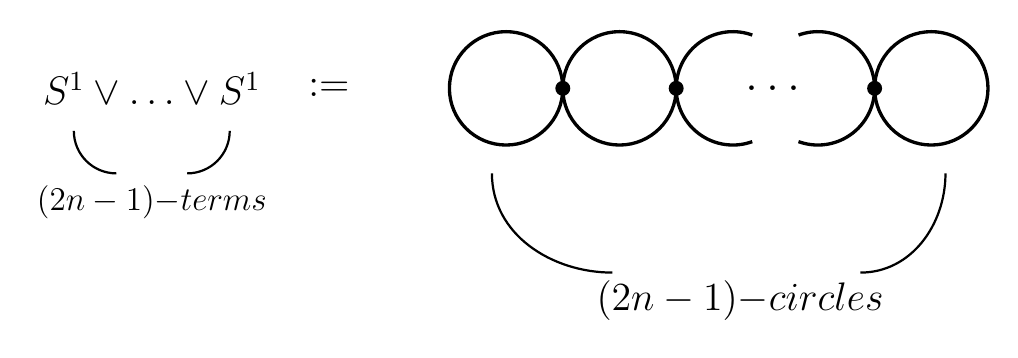
\begin{tikzpicture}[scale=0.9, very thick]
        
        
        \node at (-4, 0) {\Large $\mathbb{S}^1 \vee \dots \vee \mathbb{S}^1$};
        
        
        \draw[thick] (-5.1, -0.6) to[out=-90, in=180] (-4.5, -1.2);
        \draw[thick] (-2.9, -0.6) to[out=-90, in=0] (-3.5, -1.2);
        
        
        \node at (-4, -1.6) {\large $(2n-1)\text{-terms}$};

        
        \node at (-1.5, 0) {\Large $:=$};

        
        \def\R{0.8}
        
        
        \draw (1, 0) circle (\R);
        \fill (1+\R, 0) circle (3pt);
        
        
        \draw (1+2*\R, 0) circle (\R);
        \fill (1+3*\R, 0) circle (3pt);
        
        
        \draw (1+3*\R, 0) arc (180:70:\R);
        \draw (1+3*\R, 0) arc (180:290:\R);
        
        
        \node at (1+4.7*\R, 0) {\LARGE $\dots$};
        
        
        \draw (1+6.5*\R, 0) arc (0:110:\R);
        \draw (1+6.5*\R, 0) arc (0:-110:\R);
        \fill (1+6.5*\R, 0) circle (3pt);
        
        
        \draw (1+7.5*\R, 0) circle (\R);

        
        \draw[thick] (0.8, -1.2) to[out=-90, in=180] (2.5, -2.6);
        \draw[thick] (1+7.5*\R + 0.2, -1.2) to[out=-90, in=0] (6.0, -2.6);
        
        
        \node at (4.3, -3.0) {\Large $(2n-1)\text{-circles}$};

    \end{tikzpicture}
    \caption{Wedge sum of $2n-1$ circles}
    \end{figure}
\end{itemize}
Therefore, 
$$\Pi_1(\mathbb{R}^3 \setminus X) \cong \Pi_1 (\bigvee_{i=1}^{2n-1} \mathbb{S}^1) (= F_{2n-1})$$